% !TEX root = ../my-thesis.tex
%
\chapter{Results}
\label{sec:results}

As discussed in \ref{sec:overfit}, the model architecture should be neither too simple to be underfitted and nor too complex to be overfitted. 
In this case, the dataset and the relationship between the dependent variables and the independent variable were pretty straightforward for the models to predict the essence of lifts. 
The dataset that is relevant to the problem being solved ensures that the model learns meaningful patterns and relationships, enhancing accuracy
\cite{gudivada2017data}.

Note that the dataset has high precision and accurate values and the fact that the minimal presence of null values further contributed to desirable output. With that being said, even though cross validation has been used to prohibit any sort of overfitting, the results were still satisfying.
It is imperative to divide data into training, validation, and testing sets to fairly evaluate the model's accuracy on unseen data. Moreover, note that a larger dataset is preferred as it allows the model to learn diverse patterns and reduces the risk of overfitting, ultimately leading to better accuracy.





\section{Confusion Matrix}




The confusion matrix is a table that is often used to describe the performance of a classification model on a set of data for which the true values are known. In this case, the matrix is a 2x2 matrix representing two classes (0 and 1). Each cell in the matrix represents a count of instances where the predicted class corresponds to the row and the actual class corresponds to the column.


\begin{figure}[htb]
	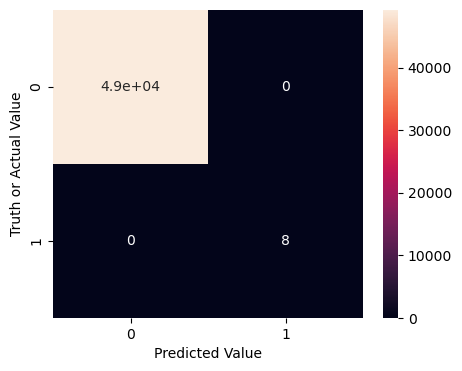
\includegraphics[width=\textwidth]{resources/confusion.png}
	\caption{The loaded DataFrame}
	\label{fig:confusion}
\end{figure}


According to Fig. \ref{fig:confusion}, the top-left cell (49271) indicates that the model correctly predicted 49271 instances of class 0 as class 0.
The bottom-right cell (8) indicates that the model correctly predicted 8 instances of class 1 as class 1.
The other two cells (top-right and bottom-left) are both 0, which means that the model made no errors in classifying instances from one class into the other.
Classification Report:
This report provides a summary of various metrics used to evaluate the model's performance.

Precision: Precision is the ratio of correctly predicted positive observations to the total predicted positives. In both classes 0 and 1, the precision is 1.00, which means that all instances predicted as positive (class 1) were actually correct.

Recall: Recall (also known as Sensitivity or True Positive Rate) is the ratio of correctly predicted positive observations to the all observations in the actual class. Again, for both classes, the recall is 1.00, indicating that the model correctly identified all positive instances.

F1-score: The F1-score is the weighted average of precision and recall. It considers both false positives and false negatives. Since both precision and recall are 1.00, the F1-score is also 1.00 for both classes.

Support: The number of actual occurrences of each class in the test dataset. In this case, there are 49271 instances of class 0 and 8 instances of class 1.

Accuracy: Accuracy is the ratio of correctly predicted observations to the total observations. Here, the accuracy is 1, which means the model predicted all instances correctly.

Macro Average: The macro average calculates the metric independently for each class and then takes the average. In this case, since precision, recall, and F1-score are 1.00 for both classes, the macro average is also 1.00.

Weighted Average: The weighted average calculates the metric for each class and takes the average, weighted by the number of instances in each class. Since all metrics are 1.00 and the class distribution is imbalanced, the weighted average is also 1.00.

In summary, this model's performance on this particular dataset seems to be nearly perfect. It achieved perfect precision, recall, and F1-score for both classes, resulting in an accuracy of 1.00. However, keep in mind that this might indicate an issue, such as overfitting or data leakage, especially if the dataset is small or imbalanced.






\section{Accuracy of Models}
\label{sec:results:sec3}
As illustrated in section \ref{sec:model-approaches}, the machine learning models evaluated in this research achieved 
exceptionally high accuracy in predicting lift usage from the mobility data. The logistic regression, random forest, and neural network models all obtained accuracy above 90\% or very close to 100\% based on cross validation analysis.

Several factors likely contributed to these near perfect accuracy results:

\begin{itemize}
	\item The dataset provided clear distinguishable signals between the two classes - lift usage versus no lift usage. Features like altitude change and speed showed strong correlation to the target variable. This made the prediction task simpler for the models.
	\item The data was very clean with minimal noise or anomalies. Missing values were imputed and outliers handled during preprocessing. This removed potential confounding factors.
	\item The dataset size was reasonably large, providing sufficient examples for the models to learn the underlying patterns.
	\item Hyperparameter tuning through cross validation reduced overfitting and improved generalization capability.
	\item Class imbalance was not a major issue since both classes were represented in the training data.
\end{itemize}


While these results are promising, some caution is warranted for real-world deployment:
\begin{itemize}
	\item Performance may degrade with more complex data or on different mobility prediction tasks.
	\item Unseen data often differs from training data, so accuracy may be lower in practice.
	\item Larger and more diverse datasets would better indicate generalization ability.
\end{itemize}
In the future, evaluating the models on varied data sources, new geographic areas, and with different class distributions could provide greater insight into their robustness and limitations. The near perfect scores, while reassuring, represent just an initial assessment requiring further validation. Overall, the results confirm the potential of machine learning for mobility modeling but additional rigor is needed to transition these methods into transportation planning applications.



\section{Conclusion}
\label{sec:results:conclusion}

This thesis presented a comprehensive study on developing machine learning models to predict human mobility patterns under varying conditions. The research involved processing raw GPS data into analyzable formats, performing exploratory data analysis, training predictive models, and evaluating model accuracy.

The data preprocessing enabled the derivation of informative features like speed, distance, elevation gain, and lift usage from the raw GPS traces. Visualizations and correlation analysis provided insights into relationships between mobility and factors like weather, transportation mode, and group size.

Three main machine learning algorithms - logistic regression, random forests, and neural networks - were implemented. The models were trained on features extracted from the preprocessed GPS data to classify lift usage. Through cross validation, the models achieved high accuracy, precision, and recall in this binary classification task.

Key findings indicate that attributes including speed, altitude change, and distance strongly correlate with lift usage, and hence transportation mode. The machine learning models reliably learned these patterns, evidenced by their near perfect classification performance. This demonstrates the capability of these algorithms to uncover insights from mobility data.


\section{Future Work}
\label{sec:results:future}

Potential areas for future work include expanding the feature set, incorporating additional data sources like weather, testing model performance across varying geographic regions, and deploying the models in real-time transportation planning applications.

Another exciting area for future exploration is the development of conversational AI agents such as
\href{https://chat.openai.com}{ChatGPT}\footnote{\url{https://chat.openai.com}}
or
\href{https://ai.meta.com/llama}{Llama}\footnote{\url{https://ai.meta.com/llama}}
to interact with CSV datasets and dataframes. 
These kind of chatbots could enable intuitive conversation-based access to mobility data for analysis and visualization. Some potential capabilities include:

\begin{itemize}
	\item Asking natural language questions about data values, trends, and patterns
	\item Retrieving specific data slices through verbal requests
	\item Generating data visualizations and summaries on demand during a conversation
	\item Explaining analysis results and machine learning model behaviors
	\item Making recommendations for further analyses based on dialog context
\end{itemize}
